
\chapter{The ATLAS Experiment at the Large Hadron Collider}
\label{chap:experiment}

In order to test the theoretical predictions and models in high energy physics in the 21st century it requires experimental setups that are unprecedented in its size and complexity.

The \emph{Large Hadron Collider} (LHC) \Rnote{}{add reference} is the most powerful particle accelerator to date and was designed and built for more than two decades starting in the early 1980s by more than $10000$ international researchers, engineers, and technicians from more than $100$ different countries. It remains the most recent large-scale upgrade to the accelerator complex at CERN, the European Organization for Nuclear Research, and allows to measure collision events at unprecedented energies.

The ATLAS detector\Rnote{}{add reference} is one of the two general purpose detectors measuring the collision events produced by the LHC. It is designed to measure a broad range of physics processes with a specific focus on observing and measuring the Higgs boson.\Mnote{Maybe leave this sentence for the ATLAS chapter} This chapter provides an overview of the LHC, followed by a detailed description of the ATLAS detector and its various subcomponents.

\Minote{}{Mention previous experiments? Tevatron, ...other?}
\Rinote{}{Improve by focusing more on the ATLAS detector in the introduction}
\Rinote{}{Add a mention that this is only a rough overview and there is much more to it.}

\section{The Large Hadron Collider}
In order to produce collision events at the highest energies, circular accelerators are utilized to be able to increase the particles' energy step-wise. The two major technical components are \emph{radiofrequency cavities} (RF cavities) with oscillating electromagnetic field to accelerate the particles as well as organizing them in so-called \emph{bunches}\footnote{RF cavities oscillate at a given frequency. Particles arriving early (late), will be decelerated (accelerated) so that the particles are kept together in discrete packages called bunches.} and magnet systems to bend, steer, and focus the particles' trajectories. The peak particle energy reached by a hadron collider is thereby limited by the maximum field strength that can be provided by the bending magnets.

The LHC is placed in a near-circular tunnel\footnote{The same tunnel was used by the former LEP collider \cites{LEPDesignReport}.} \SI{100}{\m} underground below the France-Switzerland border close to Geneva (Switzerland). It has a circumference of \SI{26.7}{\km} and collides protons in its main mode of operation. Proton bunches are accelerated with 16 RF cavities oscillating at \SI{400}{\mega\hertz} in two close-by rings to form counter-rotating beams. During operation, the LHC allows to contain a maximum of 2808 bunches separated by a bunch spacing of \SI{25}{\ns} and with about \SI{e11}{protons} in each bunch, which results in a design instantaneous luminosity of $\mathcal{L} = \SI{e34}{\per\cm\per\s}$.\footnote{The exact bunch structure of the LHC can vary between different data-taking cycles. See also \cref{sec:run-2-data-taking}}
More than 1200 superconducting twin-bore dipole magnets are used to force the particle beams on a curved trajectory.
They are designed to reach field strengths of up to \SI{8.33}{\tesla}, leading to a design centre-of-mass energy of $\sqrt{s} = \SI{14}{\TeV}$. More than 400 quadrupole magnets are used to ``squeeze'' the beams to increase the particle density within each bunch, which is especially important before the beams are made to collide at one of the four main \emph{interaction points} (IP). Each IP is surrounded by large detector systems that are optimized and designed to measure different physics processes as precisely as possible.
The ATLAS and CMS \cite{CMS-TDR-08-001} experiments are general purpose detectors, designed to measure a large variety of physics processes; the LHCb\footnote{Large Hadron Collider beauty} experiment \cite{1748-0221-3-08-S08005} is dedicated to measuring processes that involve $b$-quarks; and ALICE\footnote{A Large Ion Collider Experiment} \cite{1748-0221-3-08-S08002} focuses on the analysis of heavy-ion collisions.\footnote{There are other smaller experiments operating at the LHC: the TOTEMd (Total Elastic and Diffractive Cross Section Measurement) \cite{1748-0221-3-08-S08007} and LHCf (Large Hadron Collider forward) \cite{1748-0221-3-08-S08006} experiments study scattering processes close to the beam line and the MoEDAL (Monopole and Exotics Detector at the LHC) experiment \cite{1742-6596-631-1-012014} is dedicated to the search for magnetic monopols.}

In so-called \RunOne of the LHC, that took place between 2011 and 2012, protons were collided at $\sqrt{s} = 7\,\TeV$ and $\sqrt{s} = 8\,\TeV$, respectively. \RunTwo of the LHC refers to the data-taking period between 2015 and 2018 and delivered collisions at $\sqrt{s} = \SI{13}{\TeV}$. After a technical shutdown between 2018 and 2022, the LHC is expected to continue to operate with \RunThr at a centre-of-mass energy of at least $\sqrt{s} = \SI{13}{\TeV}$.\Rnote{}{What is the actual energy that will be used?}
The data recorded by the ATLAS experiment in \RunTwo is analyzed throughout this Thesis. Further details are given in \cref{sec:run-2-data-taking}.



\subsection{The accelerator complex}
Before the protons enter the LHC, they pass through a sophisticated chain of smaller accelerators, as depicted in \cref{fig:accelerator-complex}.
Starting from a bottle of hydrogen gas, the protons are obtained from ionizing hydrogen atoms and are first accelerated in the linear accelerator \emph{Linac2} (Linear accelerator 2)\footnote{Starting in 2020, Linac2 will be replaced by a new linear accelerator, Linac4 (Linear accelerator 4). More information can be found in \ccite{CERN-AB-2006-084}.}. This is followed by three synchrotrons that have an increasingly larger circumference and increase the energy of the proton beams step-wise: The \emph{BOOSTER} (Proton Synchrotron Booster), the \emph{PS} (Proton Synchrotron), and the \emph{SPS} (Super Proton Synchrotron). The proton beams from the SPS have an energy of $450\,\GeV$ and are then injected into the LHC where they are further accelerated. The whole ramp-up phase until stable beams with energies of $7\,\TeV$ are made to collide takes around 45 minutes. Collision events are then recorded for about 8-10 hours until the intensity of the beams becomes too low, making it more efficient to dump the beam and start a new cycle.

\begin{figure}
    %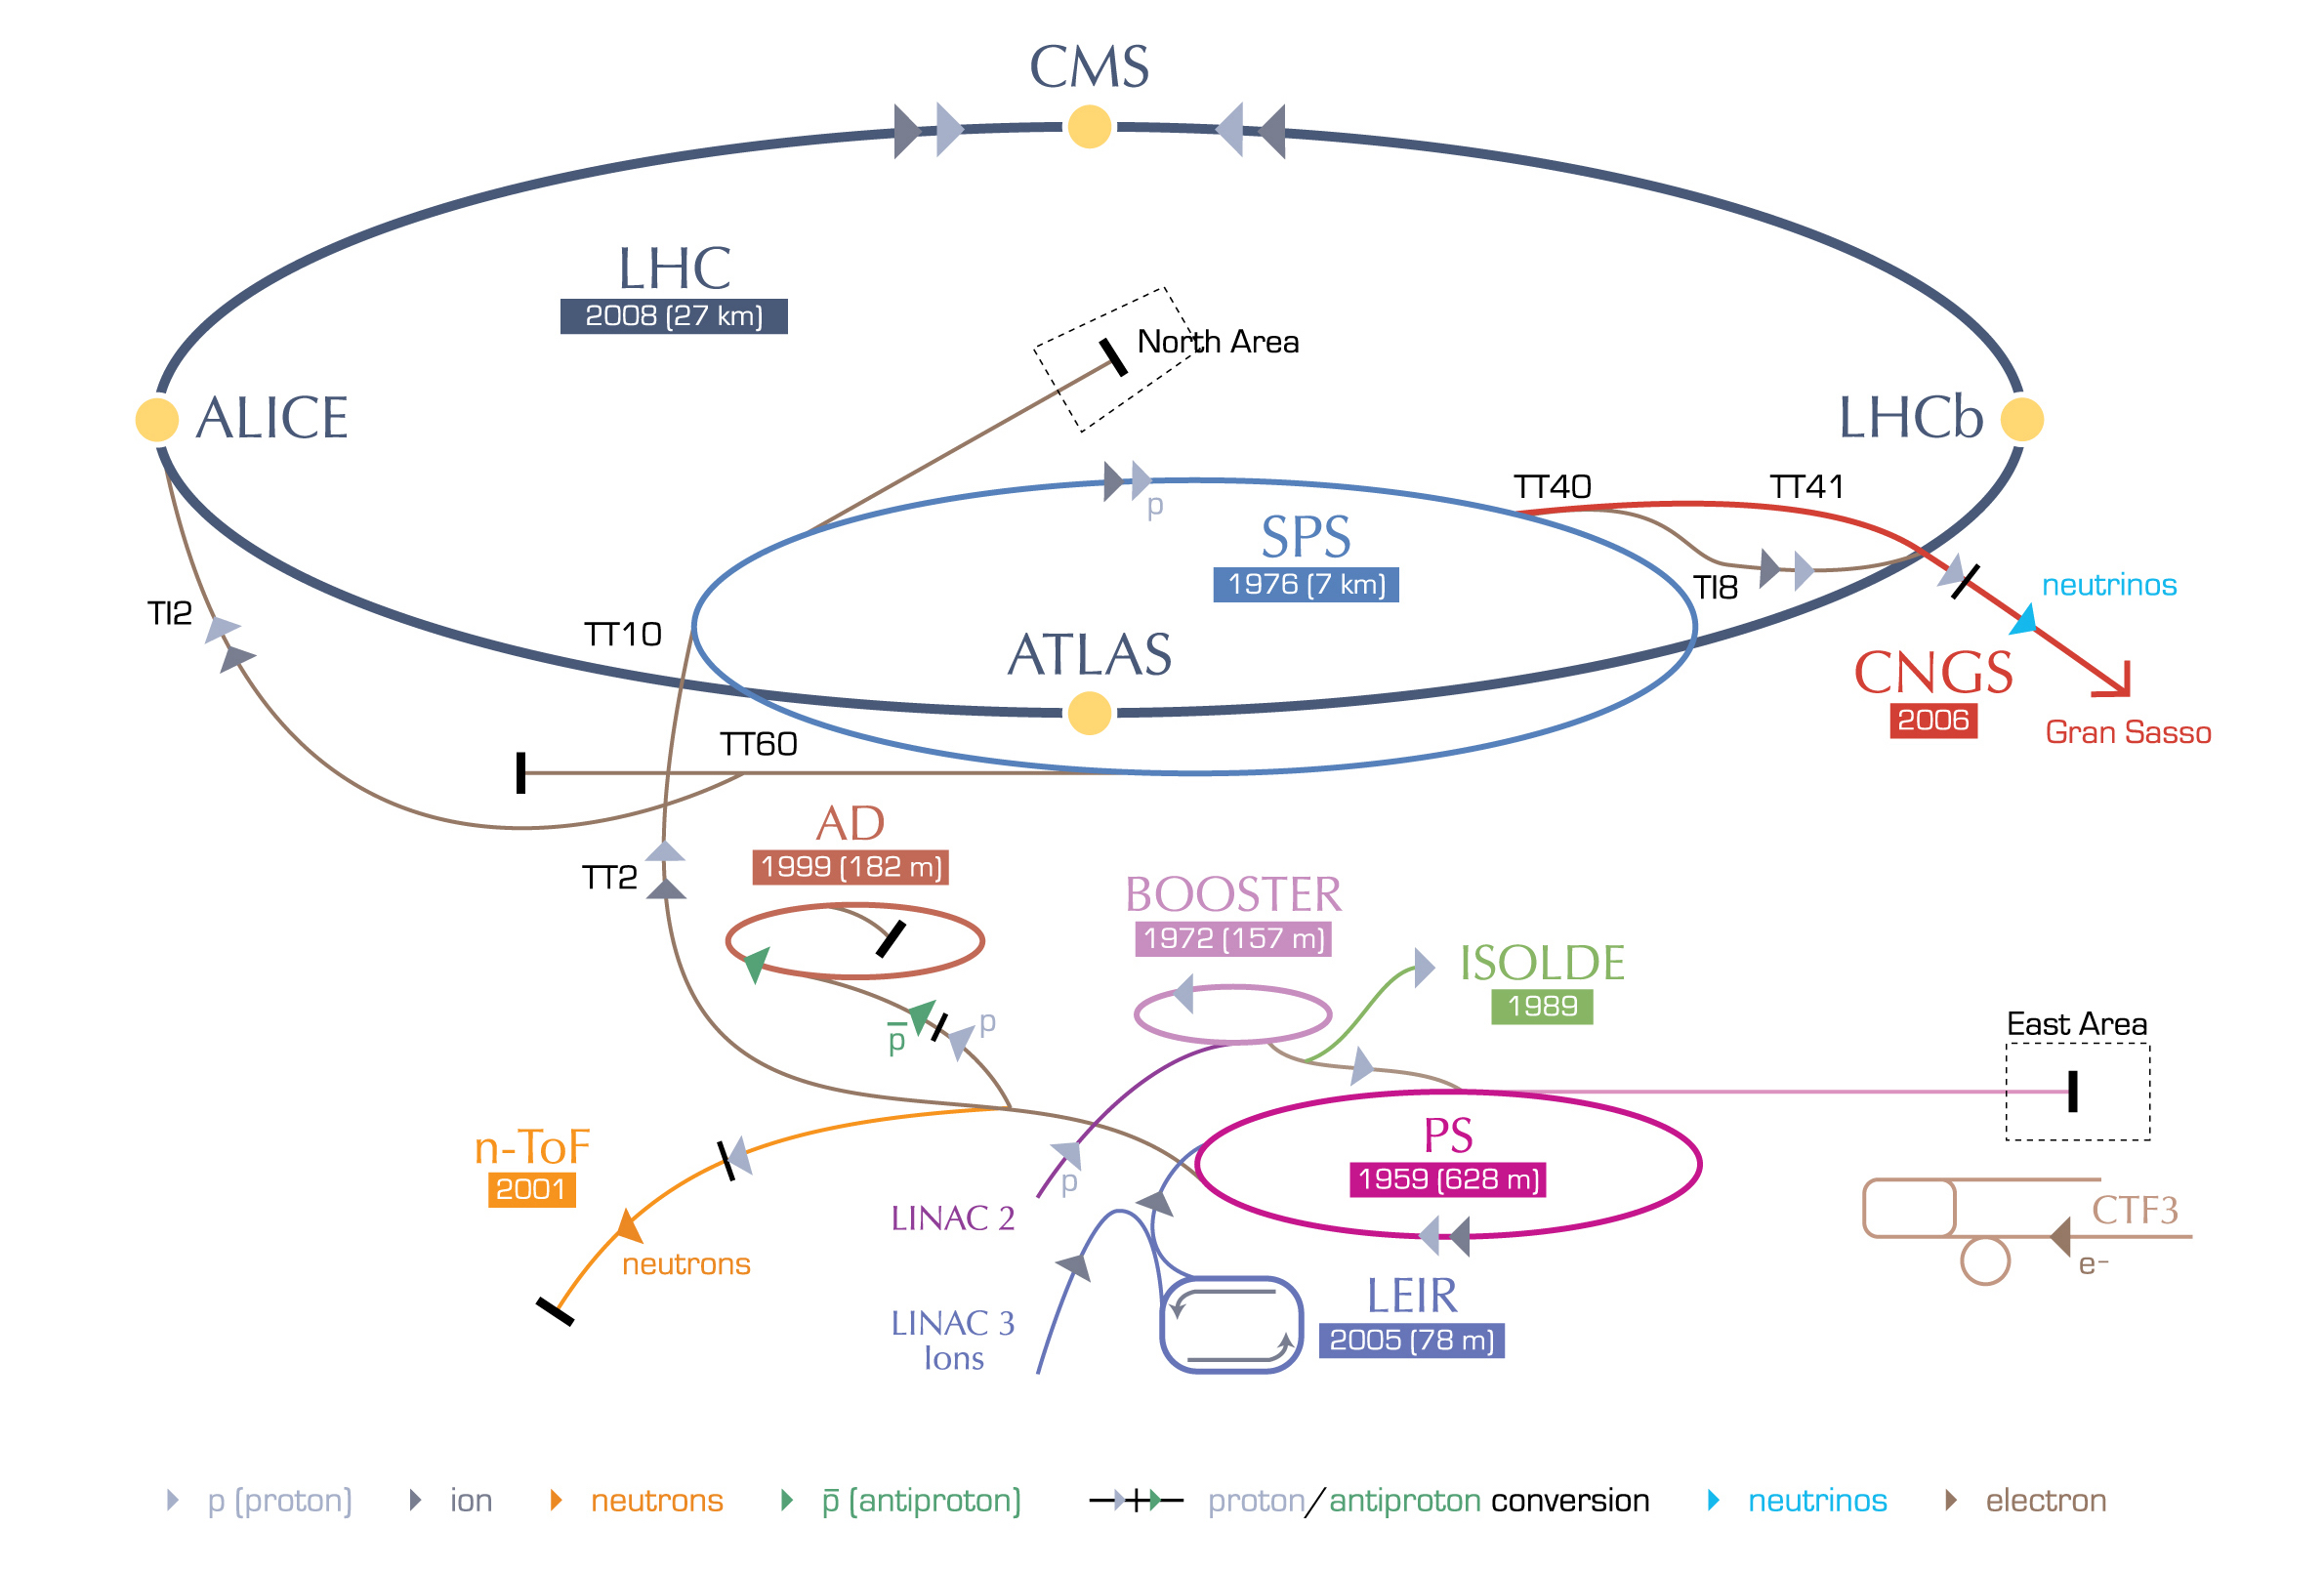
\includegraphics{figures/experiment/accelerator-complex.jpg}
    \newImageResize{figures/experiment/accelerator-complex.jpg}
    \caption[Schematic of the ATLAS detector showing the various subsystems.]{Schematic of the ATLAS detector showing the various subsystems. Adapted from \ccite{Christiane:1260465}.}
    \label{fig:accelerator-complex}
\end{figure}









\section{The ATLAS experiment}

Mention collaboration

The ATLAS detector~\cite{PERF-2007-01} ... \\

Mention coordinate system

The following describes the different components from its innermost layer to the outermost.

Different subsystems are used for triggering on interesting physics events. The trigger system is described in THIS section.

For more details on the individual subsystems the reader is referred to Ref[].

More details are given for the calorimeter system as it is the crucial component to measure the noise term of the JER presented in \cref{chap:objects}.




\begin{figure}
    \newImageResize{figures/experiment/ATLASdetector.jpg}
    \caption[Schematic of the ATLAS detector showing the various subsystems.]{Schematic of the ATLAS detector showing the various subsystems. Taken from \ccite{PERF-2007-01}.}
    \label{fig:ATLASlayout}
\end{figure}

\subsection{The Inner Detector}
\label{subsec:inner-detector}
The inner detector enables the reconstruction of charged-particle tracks stemming from the collision events by recognizing patterns in the measured particle positions often referred to as \emph{hits}. The tracks are used for impact parameter determination, primary and secondary vertexing, as well as momentum measurements. The latter is made possible by the particles' curved trajectory within a magnetic field.
Charged particle hits are detected by layers of different silicon-based semiconductor detectors as well as gaseous ionization tubes.

A schematic view of the inner detector is shown in \cref{fig:ATLASinnerdetector}.
In the barrel region the tracking detectors are arranged in cylinders around the beam axis, while in the end-cap regions, the different layers are placed on disks perpendicular to the beam axis.
The inner detector covers a range of \absetaST{2.5} and is immersed in a \SI{2}{\tesla} magnetic field that is provided by a \SI{5.8}{\m} long solenoid magnet.
The four innermost layers consist of \emph{silicon pixel} detectors that provide four space points for each charged particle. The first layer, the insertable $b$-layer \cite{ATLAS-TDR-19,PIX-2018-001}, was installed for \RunTwo of the LHC and is especially important for the reconstruction of the interaction vertices.
Four (nine) layers of \emph{silicon-microstrip} detectors in the barrel (each end-cap) region are arranged at different angles to provide additional four space points.
The fine granularity of the pixel and microstrip sensors provide high-precision measurements of particle hits with intrinsic resolutions in $R$-$\phi \times z$ of $10 \times 115\,\mu\text{m}$ and $17 \times 580\,\mu\text{m}$, respectively.

For on average 36 additional hits at longer track lengths, the \emph{Transition Radiation Tracker} (TRT) consists of a large number of straw tubes filled with xenon-based gas. The TRT covers a range of \absetaST{2.0} and provides information in the $R$-$\phi$ plane only with a resolution of \SI{130}{\micro\meter}.
Apart from the position measurement, the TRT also detects the amount of transition radiation produced by a charged particle, which helps to differentiate electrons from charged pions.
%Apart from the position measurement, the TRT is sensitive to the Lorentz factor of charged particles, by measuring the amount of transition radiation. In combination with a momentum measurement this provides the ability to compute the mass of particles and thus, gives additional information to differentiate electrons from charged pions.

\begin{figure}
    %\resizebox{\textwidth}{!}{
    \subfloat[central region]{
        \newImageScale{figures/experiment/ATLASinnerdetector.pdf}{.105}
    }
    \subfloat[end-cap region]{
        \newImageScale{figures/experiment/ATLASinnerdetectorendcap.png}{.095}
    }
 %   }
    \caption{Schematic of the ATLAS inner detector in the (a) the central region and (b) the end-cap region. Taken from Refs.~\cite{ATL-PHYS-PUB-2015-009} and \cite{PERF-2007-01}, respectively.}
    \label{fig:ATLASinnerdetector}
\end{figure}


\subsection{The Calorimeter System}
\begin{figure}
    \newImageScale{figures/experiment/ATLAScalorimeters.jpg}{.3}
    \caption[Schematic of the ATLAS calorimeters showing the different subcomponents.]{Schematic of the ATLAS calorimeters showing the different subcomponents. Taken from \ccite{PERF-2007-01}.}
    \label{fig:ATLAScalorimeters}
\end{figure}

\begin{figure}
    \subfloat[]{
        \newImageResizeCustom{figures/experiment/barrel_module.png}{0.55}
    }
    \subfloat[]{
        \newImageResizeCustom{figures/experiment/tile_module_readout.png}{0.45}
    }
    \caption{(a) Schematic of a single module of the electromagnetic calorimeter illustrating the different layers with their changing granularity. (b) Schematic of a single module of the hadronic tile calorimeter showing the different optical readout channels. Taken from \ccite{PERF-2007-01}.}
    \label{fig:ATLASmodules}
\end{figure}


\begin{itemize}
    \item Be more detailed here as I'm looking into noise term measurements
\end{itemize}

\subsection{The Muon Spectrometer}
Muons are minimum-ionizing and escape the calorimeter system. Therefore, a large muon spectrometer forms the outermost part of the ATLAS detector. It serves two main purposes: measuring track hits for muon reconstruction as well as providing fast information to the trigger system.

\Cref{fig:ATLASmuonspectrometer} shows the muon spectrometer with large superconducting toroid magnets in between of several chambers that detect the muon's ionization energy.
The 8 barrel toroid magnets and 16 end-cap magnets cover the range of \absetaST{1.4} and \absetaBT{1.6}{2.7}, respectively. They provide magnetic bending power of \numrange{0.5}{1}\,T to measure the muons' momenta. Precision-tracking chambers operate with an argon-based mixture and are arranged in three layers in both the barrel and end-cap region. They cover a range of \absetaST{2.7} and mostly consist of \emph{Monitored Drift Tubes}. Only the innermost layer in the region \absetaBT{2}{2.7} is made out of multiwire proportional chambers called \emph{Cathode Strip Chambers} that are more resistant against radiation damage. The detector chambers with fast readouts consist of \emph{Resistive Plate Chambers} (RPC) in the central-region within \absetaST{1.05} and \emph{Thin Gap Chambers} in the end-cap regions at \absetaBT{1.05}{2.4}. They provide information about traversing muons to the L1 trigger system within \numrange{15}{25}\,ns.

%The RPCs are gaseous parallel electrode-plates without a wire and 


\begin{figure}
    \newImageScale{figures/experiment/ATLASmuondetector.png}{.15}
    \caption{Schematic of the ATLAS muon spectrometer. Taken from \ccite{PERF-2007-01}.}
    \label{fig:ATLASmuonspectrometer}
\end{figure}



\subsection{Trigger System}

\subsection{Detector Simulation}


\section{Data Taking during 2015-2018}
\label{sec:run-2-data-taking}
\begin{itemize}
    \item Plot of luminosity collection
    \item Brief explanation of pile-up and pile-up distribution plot
\end{itemize}

